\section{Experiments}
\label{sec:eval}

The comparisons below are the ones that fix the default gate.
\S\ref{sec:eval-full} is the control-plane model, the per-host token ablation, the cross-model forest, and the branching sweeps.

\paragraph{Setup.}
GPU runs use vLLM on four A100-SXM4 40GB GPUs, \texttt{bfloat16} weights, temperature $0$, and prefix caching on.
The prefill gate is measured on Qwen3-8B at $\mathrm{tp}{=}1$: GSM8K with $n{=}16$ and $D{=}512$, and the first $32$ MATH-500 problems at level $\ge 4$ with $D{=}1024$.
The KV comparison is the full GSM8K test ($n{=}1319$) on Qwen3-14B at $\mathrm{tp}{=}2$.
A math answer counts when the final number matches the reference.
Any-finished asks that some full-budget branch match; the winner column in \S\ref{sec:eval-ablate} asks that the committed spine match.

\begin{table*}[t]
\centering
\caption{Main results.
The GSM8K block is Qwen3-8B, $k{=}16$, $D{=}512$.
One $\tau_{\mathrm{pre}}$ cuts prefill for every host (\Cref{prop:host}); any-finished stays $16/16$.
The MATH-500 block is the same model, $n{=}32$, $D{=}1024$, $\tau_{\mathrm{dec}}{=}0.45$.
Dropping every $s{<}\tau_{\mathrm{dec}}$ before the kernel is \eqref{eq:drej}.
The probe is \eqref{eq:dec} at $t_0{=}128$.
The last row is Qwen3-14B, $n{=}1319$, median peak KV.}
\label{tab:main}
\scriptsize
\setlength{\tabcolsep}{5pt}
\begin{tabular}{@{}llrrrr@{}}
\toprule
 & & admit & prefill & time (s) & any \\
\midrule
\multicolumn{6}{@{}l}{\emph{GSM8K.} Hosts alone share the prefill; the gate moves it.} \\
ESC / SR / DPTS & no $\tau_{\mathrm{pre}}$ & $16$ & $5008$ & $16.49$ / $13.29$ / $11.87$ & $16/16$ \\
ESC / SR / DPTS & $\tau_{\mathrm{pre}}{=}0.15$ & $12$ & \win{$3848$} & \win{$14.45$} / $12.53$ / $11.57$ & $16/16$ \\
ESC / SR / DPTS & $\tau_{\mathrm{pre}}{=}0.45$ & $8$ & \win{$2768$} & \win{$10.95$} / $10.95$ / $10.96$ & $16/16$ \\
\midrule
\multicolumn{6}{@{}l}{\emph{MATH-500.} A probe restores the branches \eqref{eq:drej} drops.} \\
full fan-out &  & $16$ & --- & $104.1$ & $20/32$ \\
drop $s{<}\tau_{\mathrm{dec}}$ & \eqref{eq:drej} & --- & --- & $52.1$ & \botn{$13/32$} \\
probe $t_0{=}128$ & \eqref{eq:dec} & --- & --- & \win{$73.2$} & \win{$20/32$} \\
\midrule
\multicolumn{6}{@{}l}{\emph{Qwen3-14B spine.} $M_{\mathrm{spine}}/M_{\mathrm{APC}}=0.72\times$ at accuracy $0.845$ vs.\ $0.844$.} \\
\bottomrule
\end{tabular}
\end{table*}

\paragraph{Prefill is host-invariant.}
\Cref{tab:main} is \Cref{prop:host} on the GPU.
ESC, Speculative Rejection, and DPTS alone each prefill $5008$ tokens, because each score is computed from tokens that already reside.
They differ only in $D^{+}$: a $512$-token window, a $256$-token partial-reward horizon, and a $100$-token mini-step, which is why the times are $16.49$\,s, $13.29$\,s, and $11.87$\,s.
Placing $\tau_{\mathrm{pre}}{=}0.15$ in front of any of them admits $12$ of $16$ residuals and cuts the prefill to $3848$ tokens ($-23\%$).
Any-finished stays $16/16$.
ESC, the host that would have decoded the loop to the end of its window, falls from $16.49$\,s to $14.45$\,s.
The same gate at $0.45$ admits $8$ residuals, cuts the prefill to $2768$ tokens, and reaches $10.95$\,s on ESC, still at $16/16$ for this $k$.
It is not the default.
\Cref{tab:prefill-bar} sweeps the same ESC host across width.
At $\tau_{\mathrm{pre}}{=}0.15$ any-finished is $16/16$ at every $k\in\{4,8,16,32\}$, and the wall-clock reduction grows with the tree ($-5\%$, $-6\%$, $-12\%$, $-17\%$) because a wider fan-out contains more repeated loops.
Computed prefill falls from $1320/2624/5008/10528$ tokens to $1018/2020/3848/7968$.
Raising the prefill threshold to $0.45$ is faster at every width ($-8\%$, $-21\%$, $-34\%$, $-49\%$) and still $16/16$ at $k\ge16$, but it drops illegal text together with the loop and loses coverage at $k{=}4$ and $k{=}8$.
The default is the cutoff that satisfies \eqref{eq:sep-pre} at every $k$.

\paragraph{End-to-end efficiency under the default gate.}
\Cref{tab:e2e-esc,tab:e2e-plugin} expand the same GSM8K branching mix into the full host comparison.
Under ESC, $\tau_{\mathrm{pre}}{=}0.15$ cuts wall-clock by $5\%$, $6\%$, $12\%$, and $17\%$ as $k$ grows from $4$ to $32$, because a wider fan-out contains more repeated loops that never enter the kernel.
Computed prefill falls from $1320/2624/5008$ to $1018/2020/3848$ tokens at $k\le16$.
Any-finished stays within one problem of the host baseline; the committed-spine winner is unchanged at $k{=}16$ ($9/16$).
The same fixed bar plugs into Speculative Rejection and DPTS without retuning (\Cref{tab:e2e-plugin}): every host drops from $5008$ to $3848$ prefill tokens and keeps $16/16$ any-finished, while the relative time cut is largest on ESC ($12\%$), which would otherwise decode the loop to the end of its window.
Raising the bar to $0.45$ at $k{=}16$ further cuts ESC to $10.95$\,s ($-34\%$) and prefill to $2768$ tokens, still at $16/16$ any-finished; the same bar loses coverage at smaller $k$ (\Cref{tab:prefill-bar}).

\begin{table*}[t]
\centering
\caption{End-to-end efficiency on GSM8K (Qwen3-8B, branching mix, $n{=}16$, $D{=}512$, $\mathrm{tp}{=}1$, temperature $0$, prefix caching on).
ESC host with $\tau_{\mathrm{pre}}{=}0.15$.
``Winner'' is committed-spine exact match.
Time is trunk warm plus fan-out.}
\label{tab:e2e-esc}
\scriptsize
\setlength{\tabcolsep}{3.2pt}
\begin{tabular}{@{}lrrrrrr@{}}
\toprule
ESC & base & ${+}\tau_{\mathrm{pre}}{=}0.15$ & cut & any & winner & prefill \\
\midrule
$k{=}4$ & $8.62$\,s & $8.22$\,s & \win{$5\%$} & $16{\to}16/16$ & $9{\to}8$ & $1320{\to}1018$ \\
\rowcolor{tblalt}
$k{=}8$ & $10.90$\,s & \win{$10.25$\,s} & \win{$6\%$} & $16{\to}16/16$ & $8{\to}10$ & $2624{\to}2020$ \\
$k{=}16$ & $16.48$\,s & \win{$14.45$\,s} & \win{$12\%$} & $16{\to}16/16$ & $9{\to}10$ & $5008{\to}3848$ \\
\rowcolor{tblalt}
$k{=}32$ & $32.78$\,s & \win{$27.14$\,s} & \win{$17\%$} & $16{\to}16/16$ & $9{\to}9$ & $10528{\to}7968$ \\
\bottomrule
\end{tabular}
\end{table*}

\begin{table*}[t]
\centering
\caption{Same slice at $k{=}16$: one $\tau_{\mathrm{pre}}$ in front of ESC, Speculative Rejection, and DPTS.
Prefill is host-invariant (\Cref{prop:host}).
Bottom block uses $\tau_{\mathrm{pre}}{=}0.45$ (faster matched any-finished at this width only).}
\label{tab:e2e-plugin}
\scriptsize
\setlength{\tabcolsep}{3.2pt}
\begin{tabular}{@{}lrrrrrr@{}}
\toprule
$k{=}16$ & base & ${+}\tau_{\mathrm{pre}}$ & cut & any & winner & prefill \\
\midrule
ESC, $0.15$ & $16.49$\,s & \win{$14.45$\,s} & \win{$12\%$} & $16/16$ & $9{\to}9$ & $5008{\to}3848$ \\
\rowcolor{tblalt}
SR, $0.15$ & $13.29$\,s & \win{$12.53$\,s} & \win{$6\%$} & $16/16$ & $9{\to}9$ & $5008{\to}3848$ \\
DPTS, $0.15$ & $11.87$\,s & $11.57$\,s & $3\%$ & $16/16$ & $10{\to}10$ & $5008{\to}3848$ \\
\midrule
ESC, $0.45$ & $16.49$\,s & \win{$10.95$\,s} & \win{$34\%$} & $16/16$ & $9{\to}9$ & $5008{\to}$\win{2768} \\
\rowcolor{tblalt}
SR, $0.45$ & $13.29$\,s & \win{$10.95$\,s} & \win{$18\%$} & $16/16$ & $9{\to}9$ & $5008{\to}$\win{2768} \\
DPTS, $0.45$ & $11.87$\,s & \win{$10.96$\,s} & \win{$8\%$} & $16/16$ & $10{\to}9$ & $5008{\to}$\win{2768} \\
\bottomrule
\end{tabular}
\end{table*}

\begin{figure*}[t]
\centering
\resizebox{\textwidth}{!}{\begin{tikzpicture}[
  font=\scriptsize\sffamily,
  >=Latex,
  tick/.style={font=\tiny, text=black!55, inner sep=0pt},
  grid/.style={black!12, line width=0.25pt},
  ax/.style={black!55, line width=0.35pt},
  bar/.style={draw=black!45, line width=0.2pt},
]
\definecolor{ESCc}{HTML}{C48A3A}
\definecolor{t15}{HTML}{D97B2F}
\definecolor{t45}{HTML}{4A2878}

% tab:prefill-bar. Time y = 0.42 + seconds * 0.13 (0--18).
% Prefill y = 0.42 + tokens/5500 * 2.34.
% k at x = 1.35, 2.85, 4.35.
% Plugin e2e uses the same time scale.

\node[font=\tiny, anchor=west] at (0.05,3.35) {GSM8K, Qwen3-8B, $n{=}16$, $D{=}512$};

\begin{scope}[shift={(0.70,0.20)}]
  \node[font=\tiny\bfseries, anchor=west] at (0,2.95) {(a) End-to-end time};
  \foreach \y/\lab in {0.42/0, 1.20/6, 1.98/12, 2.76/18} {
    \draw[grid] (0.35,\y) -- (5.05,\y);
    \node[tick, anchor=east] at (0.28,\y) {\lab};
  }
  \draw[ax] (0.35,0.42) -- (5.05,0.42);
  \draw[ax] (0.35,0.42) -- (0.35,2.80);
  \draw[ESCc, line width=0.8pt] (1.35,1.545) -- (2.85,1.829) -- (4.35,2.637);
  \draw[t15, line width=0.8pt] (1.35,1.489) -- (2.85,1.745) -- (4.35,2.258);
  \draw[t45, line width=0.8pt] (1.35,1.446) -- (2.85,1.538) -- (4.35,1.841);
  \foreach \x/\y in {1.35/1.545, 2.85/1.829, 4.35/2.637} {\fill[ESCc] (\x,\y) circle (1.2pt);}
  \foreach \x/\y in {1.35/1.489, 2.85/1.745, 4.35/2.258} {\fill[t15] (\x,\y) circle (1.2pt);}
  \foreach \x/\y in {1.35/1.446, 2.85/1.538, 4.35/1.841} {\fill[t45] (\x,\y) circle (1.2pt);}
  \node[font=\tiny, text=t15, anchor=south] at (1.05,1.72) {$15/16$};
  \node[font=\tiny, text=t45, anchor=north] at (1.05,1.22) {$14/16$};
  \node[font=\tiny, text=t45, anchor=north] at (2.55,1.28) {$14/16$};
  \node[font=\tiny, text=black!55, anchor=south west] at (4.05,2.68) {$16/16$};
  \foreach \x/\lab in {1.35/4, 2.85/8, 4.35/16} {\node[tick] at (\x,0.22) {$k{=}\lab$};}
  \node[tick, rotate=90, anchor=south] at (-0.12,1.60) {seconds};
\end{scope}

\begin{scope}[shift={(6.15,0.20)}]
  \node[font=\tiny\bfseries, anchor=west] at (0,2.95) {(b) Computed prefill};
  \foreach \y/\lab in {0.42/0, 1.484/2.5k, 2.547/5k} {
    \draw[grid] (0.45,\y) -- (5.05,\y);
    \node[tick, anchor=east] at (0.38,\y) {\lab};
  }
  \draw[ax] (0.45,0.42) -- (5.05,0.42);
  \draw[ax] (0.45,0.42) -- (0.45,2.80);
  \draw[ESCc, line width=0.8pt] (1.35,0.982) -- (2.85,1.537) -- (4.35,2.551);
  \draw[t15, line width=0.8pt] (1.35,0.853) -- (2.85,1.279) -- (4.35,2.057);
  \draw[t45, line width=0.8pt] (1.35,0.731) -- (2.85,1.036) -- (4.35,1.598);
  \foreach \x/\y in {1.35/0.982, 2.85/1.537, 4.35/2.551} {\fill[ESCc] (\x,\y) circle (1.2pt);}
  \foreach \x/\y in {1.35/0.853, 2.85/1.279, 4.35/2.057} {\fill[t15] (\x,\y) circle (1.2pt);}
  \foreach \x/\y in {1.35/0.731, 2.85/1.036, 4.35/1.598} {\fill[t45] (\x,\y) circle (1.2pt);}
  \node[font=\tiny, text=ESCc, anchor=south] at (4.35,2.58) {$5008$};
  \node[font=\tiny, text=t15, anchor=west] at (4.42,1.98) {$3848$};
  \node[font=\tiny, text=t45, anchor=west] at (4.42,1.52) {$2768$};
  \foreach \x/\lab in {1.35/4, 2.85/8, 4.35/16} {\node[tick] at (\x,0.22) {$k{=}\lab$};}
  \node[tick, rotate=90, anchor=south] at (-0.08,1.60) {tokens};
\end{scope}

\begin{scope}[shift={(11.55,0.20)}]
  \node[font=\tiny\bfseries, anchor=west] at (0,2.95) {(c) $k{=}16$, three hosts};
  \foreach \y/\lab in {0.42/0, 1.20/6, 1.98/12, 2.76/18} {
    \draw[grid] (0.35,\y) -- (3.85,\y);
    \node[tick, anchor=east] at (0.28,\y) {\lab};
  }
  \draw[ax] (0.35,0.42) -- (3.85,0.42);
  \draw[ax] (0.35,0.42) -- (0.35,2.80);
  % ESC 17.05 / 14.14, SR 13.14 / 12.47, DPTS 11.86 / 11.49
  \fill[bar, ESCc] (0.70,0.42) rectangle (1.02,2.637);
  \fill[bar, t15] (1.08,0.42) rectangle (1.40,2.258);
  \fill[bar, ESCc] (1.85,0.42) rectangle (2.17,2.102);
  \fill[bar, t15] (2.23,0.42) rectangle (2.55,2.013);
  \fill[bar, ESCc] (3.00,0.42) rectangle (3.32,1.931);
  \fill[bar, t15] (3.38,0.42) rectangle (3.70,1.882);
  \node[font=\tiny, text=fsgain] at (1.24,2.72) {$-17\%$};
  \node[font=\tiny, text=fsgain] at (2.39,2.20) {$-5\%$};
  \node[font=\tiny, text=fsgain] at (3.54,2.02) {$-3\%$};
  \node[tick] at (1.05,0.22) {ESC};
  \node[tick] at (2.20,0.22) {SR};
  \node[tick] at (3.35,0.22) {DPTS};
  \node[tick, rotate=90, anchor=south] at (-0.12,1.60) {seconds};
\end{scope}

\fill[ESCc] (4.55,-0.38) rectangle (4.78,-0.22);
\node[font=\tiny, anchor=west] at (4.84,-0.30) {Host alone};
\fill[t15] (6.55,-0.38) rectangle (6.78,-0.22);
\node[font=\tiny, anchor=west] at (6.84,-0.30) {$\tau_{\mathrm{pre}}{=}0.15$};
\fill[t45] (9.15,-0.38) rectangle (9.38,-0.22);
\node[font=\tiny, anchor=west] at (9.44,-0.30) {$\tau_{\mathrm{pre}}{=}0.45$};
\node[font=\tiny, text=black!55, anchor=west] at (11.55,-0.30) {(c) gold $=$ host, orange $=$ $+\tau_{\mathrm{pre}}{=}0.15$};
\end{tikzpicture}
}
\caption{\textbf{Prefill threshold on GSM8K} (\Cref{tab:prefill-bar,tab:e2e-plugin,tab:plugin}).
(a)~Wall-clock under ESC. Labels are any-finished.
$\tau_{\mathrm{pre}}{=}0.45$ is $14/16$ at $k{=}4$, $15/16$ at $k{=}8$, and $16/16$ at $k{=}16$.
(b)~Computed prefill, $-23\%$ at $0.15$ and $-45\%$ at $0.45$.
(c)~The same $0.15$ threshold in front of each host at $k{=}16$. Every row stays $16/16$.}
\label{fig:eval-admit}
\end{figure*}

\paragraph{Connector payload under disaggregation.}
The same $\tau_{\mathrm{pre}}{=}0.15$ rule that cuts GPU prefill also cuts the P/D connector when the trunk is still cloned on the prefiller (\Cref{tab:connector}).
On the control-plane model ($10$ sessions, $k{=}4$, $L{=}256$, $\ell{=}32$), stock disaggregation ships $\Xfer{=}kL+\sum_i\ell_i{=}11520$ tokens.
Withholding only the loop keeps three residuals per fan-out, each still carrying the trunk on a stock prefiller, so $\Xfer{=}10{\times}3{\times}288{=}8640$ ($-25\%$) and transfer time falls from $23.0$\,ms to $17.3$\,ms.
Aliasing the trunk on top of that gate removes $L$ from both $\Work$ and $\Xfer$ (\Cref{tab:app} in \S\ref{sec:eval-app}).

\begin{table}[t]
\centering
\caption{Control-plane connector under P/D disaggregation ($10$ sessions, $k{=}4$, $L{=}256$, $\ell{=}32$).
Prefill $12\,\mu\mathrm{s}/\mathrm{token}$; transfer $2\,\mu\mathrm{s}/\mathrm{token}$.
``Loop-only'' is $\tau_{\mathrm{pre}}{=}0.15$ on a stock (non-aliased) prefiller---the accuracy-preserving gate of \Cref{tab:e2e-esc}.
``Alias$+$gate'' aliases the trunk and ships only the miss of $\Keep$.
Not GPU wall-clock.}
\label{tab:connector}
\scriptsize
\setlength{\tabcolsep}{4pt}
\begin{tabular}{@{}lrrrr@{}}
\toprule
 & APC & P/D & P/D + loop-only & Alias$+$gate \\
\midrule
Prefill tokens $\Work$ & $11520$ & \botn{$11520$} & \win{$8640$} & \win{$960$} \\
\rowcolor{tblalt}
Connector tokens $\Xfer$ & $0$ & \botn{$11520$} & \win{$8640$} & \win{$960$} \\
Transfer time & $0$ & \botn{$23.0$\,ms} & \win{$17.3$\,ms} & \win{$1.9$\,ms} \\
\rowcolor{tblalt}
Fan-out & $138.2$\,ms & \botn{$161.3$\,ms} & \win{$121.0$\,ms} & \win{$13.4$\,ms} \\
\bottomrule
\end{tabular}
\end{table}

\paragraph{Any-finished and the committed spine.}
Any-finished counts a problem when some full-budget branch matches the reference.
The winner column of \Cref{tab:ablate} counts a problem when the committed spine matches.
On this GSM8K slice the three hosts alone are all $16/16$ any-finished, while the spine matches on $9/16$ under ESC and Speculative Rejection and on $10/16$ under DPTS.
The prefill stays $5008$ tokens.
The hosts differ in decode tokens ($131072$, $98304$, $78336$) and in how many admitted residuals they stop later ($0$, $8$, $8$).
Placing $\tau_{\mathrm{pre}}{=}0.15$ in front of ESC keeps that winner at $9/16$ and cuts decode tokens to $98304$, because the four loops never start.
The same gate in front of DPTS keeps the winner at $10/16$ and finishes in $11.57$\,s; Speculative Rejection with the same gate finishes in $12.53$\,s at $9/16$.
At $0.45$ every combined row is $9/16$ on the winner: the residuals a $0.45$ prefill cutoff withholds include branches that would have matched the reference under DPTS.
Retaining one unscored child is stricter.
At the same $k$ and $\tau{=}0.45$ that policy prefills $414$ tokens and reaches $11/16$ any-finished under ESC and $9/16$ under Speculative Rejection, against $16/16$ when the eight residuals that clear the score are admitted (\S\ref{sec:eval-wide}).
The gate is a threshold on every residual, and index $0$ is held out of it.

\begin{table}[t]
\centering
\caption{GSM8K, Qwen3-8B, $n{=}16$, $D{=}512$, ESC only.
Any-finished is exact match on a full-budget branch.
$\tau_{\mathrm{pre}}{=}0.15$ drops the loop; $0.45$ also drops illegal text.
Time is trunk warm plus fan-out, in seconds.}
\label{tab:prefill-bar}
\scriptsize
\setlength{\tabcolsep}{3.0pt}
\begin{tabular}{lrrr}
\rowcolor{tblhead}
\toprule
 & $k{=}4$ & $k{=}8$ & $k{=}16$ \\
\midrule
ESC & $16/16$, $8.62$ & $16/16$, $10.90$ & $16/16$, $16.48$ \\
\rowcolor{tblalt}
\app $\tau_{\mathrm{pre}}{=}0.15$ & \win{$16/16$}, $8.22$ & \win{$16/16$}, $10.25$ & \win{$16/16$}, $14.45$ \\
\app $\tau_{\mathrm{pre}}{=}0.45$ & \botn{$14/16$}, $7.90$ & \botn{$15/16$}, $8.66$ & \win{$16/16$}, \win{$10.95$} \\
\bottomrule
\end{tabular}
\end{table}

\paragraph{The probe is the decode threshold.}
On MATH-500 at $k{=}16$, \eqref{eq:drej} drops any-finished accuracy from $20/32$ to $13/32$.
\eqref{eq:dec} with $t_0{=}128$ returns the count to $20/32$ and cuts end-to-end time from $104.1$\,s to $73.2$\,s.
The loop is the only residual that stays at $d_i{=}0$.
Illegal text is prefilled, probed, and extended when the prefix clears $0.45$, which is the separation in \eqref{eq:sep-pre}--\eqref{eq:sep-dec}.
\Cref{tab:grow} is the same rule at three widths.
Dropping every score below $\tau_{\mathrm{dec}}$ cuts any-finished from $12/32$ to $6/32$ at $k{=}4$ and from $20/32$ to $13/32$ at $k{=}16$.
Skipping only the loop is safe at every width: those branches finish $0$ for $0$.
The probe length depends on $k$.
At $k{=}16$, $t_0{=}128$ extends every illegal residual and returns $20/32$ in $73.2$\,s, with decode tokens falling from $524288$ to $393216$.
At $k{=}8$ the shorter probe is the one that holds the count ($15/32$ in $42.8$\,s, matching the full fan-out).
At $k{=}4$ neither probe recovers $12/32$; decoding the single illegal residual all the way to $D$ is the closer point ($11/32$ in $23.0$\,s).
Keeping one unscored residual instead of the eight that clear $0.45$ falls to $11/16$ under ESC and $9/16$ under Speculative Rejection (\S\ref{sec:eval-wide}).

\begin{figure*}[t]
\centering
\resizebox{\textwidth}{!}{\begin{tikzpicture}[
  font=\scriptsize\sffamily,
  >=Latex,
  tick/.style={font=\tiny, text=black!55, inner sep=0pt},
  grid/.style={black!12, line width=0.25pt},
  ax/.style={black!55, line width=0.35pt},
  mk/.style={circle, inner sep=0pt, minimum size=2.6pt},
]
\definecolor{fullc}{HTML}{3D3D3D}
\definecolor{dropc}{HTML}{B00020}
\definecolor{skipc}{HTML}{5D6D7E}
\definecolor{g64c}{HTML}{D97B2F}
\definecolor{g128}{HTML}{0B6E4F}

% Table tab:grow. y = 0.40 + count * 0.115 (0--20 of 32).
% Time y = 0.40 + seconds * 0.02091 (0--110).
% k at x = 1.6, 3.4, 5.2.

\node[font=\tiny, anchor=west] at (0.15,3.55) {MATH-500, Qwen3-8B, $n{=}32$, $D{=}1024$, $\tau{=}0.45$};

\begin{scope}[shift={(0.85,0.15)}]
  \node[font=\tiny\bfseries, anchor=west] at (0,3.05) {(a) Any-finished};
  \foreach \y/\lab in {0.40/0, 1.55/10, 2.70/20} {
    \draw[grid] (0.4,\y) -- (6.15,\y);
    \node[tick, anchor=east] at (0.32,\y) {\lab};
  }
  \draw[ax] (0.4,0.40) -- (6.15,0.40);
  \draw[ax] (0.4,0.40) -- (0.4,2.85);
  \draw[fullc, line width=0.8pt] (1.6,1.780) -- (3.4,2.125) -- (5.2,2.700);
  \draw[dropc, dashed, line width=0.7pt] (1.6,1.090) -- (3.4,1.665) -- (5.2,1.895);
  \draw[skipc, densely dotted, line width=0.8pt] (1.6,1.665) -- (3.4,2.355) -- (5.2,2.240);
  \draw[g64c, line width=0.8pt] (1.6,1.320) -- (3.4,2.240) -- (5.2,2.470);
  \draw[g128, line width=0.95pt] (1.6,1.435) -- (3.4,1.895) -- (5.2,2.700);
  \foreach \x/\y in {1.6/1.780, 3.4/2.125, 5.2/2.700} {\fill[fullc] (\x,\y) circle (1.15pt);}
  \foreach \x/\y in {1.6/1.090, 3.4/1.665, 5.2/1.895} {\fill[dropc] (\x,\y) circle (1.15pt);}
  \foreach \x/\y in {1.6/1.665, 3.4/2.355, 5.2/2.240} {\fill[skipc] (\x,\y) circle (1.15pt);}
  \foreach \x/\y in {1.6/1.320, 3.4/2.240, 5.2/2.470} {\fill[g64c] (\x,\y) circle (1.15pt);}
  \foreach \x/\y in {1.6/1.435, 3.4/1.895, 5.2/2.700} {\draw[g128, line width=0.6pt, fill=white] (\x,\y) circle (1.7pt);}
  \node[font=\tiny, text=g128, anchor=south west] at (5.28,2.62) {$20$};
  \node[font=\tiny, text=dropc, anchor=north west] at (5.28,1.82) {$13$};
  \foreach \x/\lab in {1.6/4, 3.4/8, 5.2/16} {\node[tick] at (\x,0.18) {$k{=}\lab$};}
  \node[tick, rotate=90, anchor=south] at (-0.05,1.62) {of $32$};
\end{scope}

\begin{scope}[shift={(7.55,0.15)}]
  \node[font=\tiny\bfseries, anchor=west] at (0,3.05) {(b) End-to-end time};
  \foreach \y/\lab in {0.40/0, 1.446/50, 2.491/100} {
    \draw[grid] (0.4,\y) -- (6.15,\y);
    \node[tick, anchor=east] at (0.32,\y) {\lab};
  }
  \draw[ax] (0.4,0.40) -- (6.15,0.40);
  \draw[ax] (0.4,0.40) -- (0.4,2.85);
  \draw[fullc, line width=0.8pt] (1.6,0.929) -- (3.4,1.498) -- (5.2,2.577);
  \draw[dropc, dashed, line width=0.7pt] (1.6,0.799) -- (3.4,0.935) -- (5.2,1.489);
  \draw[skipc, densely dotted, line width=0.8pt] (1.6,0.881) -- (3.4,1.268) -- (5.2,1.893);
  \draw[g64c, line width=0.8pt] (1.6,0.902) -- (3.4,1.278) -- (5.2,1.916);
  \draw[g128, line width=0.95pt] (1.6,0.916) -- (3.4,1.305) -- (5.2,1.910);
  \foreach \x/\y in {1.6/0.929, 3.4/1.498, 5.2/2.577} {\fill[fullc] (\x,\y) circle (1.15pt);}
  \foreach \x/\y in {1.6/0.799, 3.4/0.935, 5.2/1.489} {\fill[dropc] (\x,\y) circle (1.15pt);}
  \foreach \x/\y in {1.6/0.881, 3.4/1.268, 5.2/1.893} {\fill[skipc] (\x,\y) circle (1.15pt);}
  \foreach \x/\y in {1.6/0.902, 3.4/1.278, 5.2/1.916} {\fill[g64c] (\x,\y) circle (1.15pt);}
  \foreach \x/\y in {1.6/0.916, 3.4/1.305, 5.2/1.910} {\draw[g128, line width=0.6pt, fill=white] (\x,\y) circle (1.7pt);}
  \node[font=\tiny, text=fullc, anchor=south] at (5.2,2.62) {$104.1$};
  \node[font=\tiny, text=g128, anchor=north] at (5.2,1.82) {$73.2$};
  \foreach \x/\lab in {1.6/4, 3.4/8, 5.2/16} {\node[tick] at (\x,0.18) {$k{=}\lab$};}
  \node[tick, rotate=90, anchor=south] at (-0.18,1.62) {seconds};
\end{scope}

\fill[fullc] (0.85,-0.42) rectangle (1.08,-0.26);
\node[font=\tiny, anchor=west] at (1.12,-0.34) {Full};
\draw[dropc, dashed, line width=0.7pt] (2.05,-0.34) -- (2.45,-0.34);
\node[font=\tiny, anchor=west] at (2.50,-0.34) {Drop $s{<}\tau$};
\draw[skipc, densely dotted, line width=0.8pt] (4.55,-0.34) -- (4.95,-0.34);
\node[font=\tiny, anchor=west] at (5.00,-0.34) {Skip loops};
\fill[g64c] (6.85,-0.42) rectangle (7.08,-0.26);
\node[font=\tiny, anchor=west] at (7.12,-0.34) {Grow $t_0{=}64$};
\draw[g128, line width=0.7pt, fill=white] (9.35,-0.34) circle (1.8pt);
\node[font=\tiny, anchor=west] at (9.55,-0.34) {Grow $t_0{=}128$};
\end{tikzpicture}
}
\caption{\textbf{Probe admission on MATH-500} (\Cref{tab:grow}).
Dropping every $s{<}\tau$ is the fast, low-count curve.
Grow $t_0{=}128$ returns to $20/32$ at $k{=}16$ and cuts $104.1$\,s to $73.2$\,s.
At $k{=}8$, grow $t_0{=}64$ is $15/32$ in $42.8$\,s, matching the full fan-out.}
\label{fig:eval-grow}
\end{figure*}

\begin{table}[t]
\centering
\caption{MATH-500 level $\ge 4$, Qwen3-8B, $n{=}32$, $D{=}1024$.
Each cell is any-finished and seconds.
``Drop $s{<}\tau$'' is \eqref{eq:drej}.
``Grow $t_0$'' is \eqref{eq:dec}: loops stay at $d_i{=}0$; every other low score is probed and continues to $D$ only if $s'_i\ge 0.45$.}
\label{tab:grow}
\scriptsize
\setlength{\tabcolsep}{3.0pt}
\begin{tabular}{lrrr}
\rowcolor{tblhead}
\toprule
 & $k{=}4$ & $k{=}8$ & $k{=}16$ \\
\midrule
Full fan-out & $12/32$, $25.3$ & $15/32$, $52.5$ & $20/32$, $104.1$ \\
\rowcolor{tblalt}
Drop $s{<}\tau$ & $6/32$, $19.1$ & $11/32$, $25.6$ & $13/32$, $52.1$ \\
Skip loops only & $11/32$, $23.0$ & $17/32$, $41.5$ & $16/32$, $71.4$ \\
\rowcolor{tblalt}
Grow $t_0{=}64$ & $12/32$, $24.0$ & \win{$15/32$}, $42.8$ & $18/32$, $72.7$ \\
Grow $t_0{=}128$ & $9/32$, $24.8$ & $14/32$, $43.3$ & \win{$20/32$}, $73.2$ \\
\bottomrule
\end{tabular}
\end{table}

\paragraph{The spine is the live set.}
On Qwen3-14B the committed spine matches APC accuracy at $0.72\times$ the median peak KV (\Cref{tab:gsm}).
The same ratio stays in $0.72$--$0.75\times$ on six model families (\Cref{fig:eval-multi}).
Over three Tree-of-Thoughts turns the same gate runs before each fan-out (\S\ref{sec:eval-mt}).
On Game of 24 the turns propose an equation, continue on the cards that remain, and write the expression that uses all four cards; on GSM8K they set up the algebra, rewrite the previous step, and collect the final number.
Across $16$ problems, three turns, and $k{=}4$, that is $192$ residuals, of which \plus{} prefills $48$.
End-to-end time on Qwen3-8B falls from $2.48$\,s to $1.91$\,s on GSM8K and from $2.15$\,s to $1.52$\,s on Game of 24.
Expand time is $7.9$--$10.6\times$ below APC (\Cref{tab:mt-split}).
Accuracy stays with APC on GSM8K and rises on Game of 24, from $6/16$ to $9/16$ on Qwen3-4B and from $9/16$ to $10/16$ on Qwen3-8B (\Cref{tab:mt,fig:eval-mt}).

\begin{figure*}[t]
\centering
\resizebox{\textwidth}{!}{\begin{tikzpicture}[
  font=\scriptsize\sffamily,
  bar/.style={draw=black!65, line width=0.22pt},
  >=Latex,
]
\definecolor{Rec}{HTML}{F8E6A0}
\definecolor{APC}{HTML}{E8B86D}
\definecolor{FS}{HTML}{D97B2F}
\definecolor{FSp}{HTML}{4A2878}

\fill[Rec] (4.10,7.48) rectangle (4.32,7.64);
\node[font=\tiny, anchor=west] at (4.36,7.56) {Recompute};
\fill[APC] (5.95,7.48) rectangle (6.17,7.64);
\node[font=\tiny, anchor=west] at (6.21,7.56) {APC};
\fill[FS] (7.15,7.48) rectangle (7.37,7.64);
\node[font=\tiny, anchor=west] at (7.41,7.56) {\sys};
\fill[FSp] (8.95,7.48) rectangle (9.17,7.64);
\node[font=\tiny, anchor=west] at (9.21,7.56) {\plus};

% --- Qwen3-4B ---
\begin{scope}[shift={(0.00,3.75)}]
  \node[font=\tiny\bfseries] at (2.20,3.41) {Qwen3-4B};
  \draw[black!12] (0.44,0.300) -- (4.18,0.300);
  \node[font=\tiny, text=black!45, anchor=east] at (0.38,0.300) {0};
  \draw[black!12] (0.44,1.119) -- (4.18,1.119);
  \node[font=\tiny, text=black!45, anchor=east] at (0.38,1.119) {1.5k};
  \draw[black!12] (0.44,1.939) -- (4.18,1.939);
  \node[font=\tiny, text=black!45, anchor=east] at (0.38,1.939) {3.0k};
  \draw[black!12] (0.44,2.758) -- (4.18,2.758);
  \node[font=\tiny, text=black!45, anchor=east] at (0.38,2.758) {4.5k};
  \draw[black!55] (0.44,0.30) -- (4.18,0.30);
  \draw[black!55] (0.44,0.30) -- (0.44,3.25);
  \fill[bar, Rec] (0.360,0.30) rectangle (0.660,2.739);
  \fill[bar, APC] (0.730,0.30) rectangle (1.030,1.126);
  \fill[bar, FS] (1.100,0.30) rectangle (1.400,0.907);
  \fill[bar, FSp] (1.470,0.30) rectangle (1.770,0.907);
  \node[font=\tiny, inner sep=0.2pt, fill=white, fill opacity=0.85, text opacity=1] at (0.510,2.879) {4464};
  \node[font=\tiny, inner sep=0.2pt, fill=white, fill opacity=0.85, text opacity=1] at (0.880,1.266) {1512};
  \node[font=\tiny, inner sep=0.2pt, fill=white, fill opacity=0.85, text opacity=1] at (1.435,1.047) {1112};
  \draw[black!75, line width=0.35pt] (0.880,1.126) -- (0.880,1.546);
  \draw[black!75, line width=0.35pt] (0.880,1.546) -- (1.250,1.546);
  \draw[black!75, line width=0.35pt] (1.250,1.546) -- (1.250,0.907);
  \node[font=\tiny\bfseries] at (1.065,1.696) {$0.74\times$};
  \node[font=\tiny, text=black!55] at (0.915,0.12) {GSM8K};
  \fill[bar, Rec] (2.280,0.30) rectangle (2.580,1.972);
  \fill[bar, APC] (2.650,0.30) rectangle (2.950,1.003);
  \fill[bar, FS] (3.020,0.30) rectangle (3.320,0.732);
  \fill[bar, FSp] (3.390,0.30) rectangle (3.690,0.732);
  \node[font=\tiny, inner sep=0.2pt, fill=white, fill opacity=0.85, text opacity=1] at (2.430,2.112) {3060};
  \node[font=\tiny, inner sep=0.2pt, fill=white, fill opacity=0.85, text opacity=1] at (2.800,1.143) {1287};
  \node[font=\tiny, inner sep=0.2pt, fill=white, fill opacity=0.85, text opacity=1] at (3.355,0.872) {791};
  \draw[black!75, line width=0.35pt] (2.800,1.003) -- (2.800,1.423);
  \draw[black!75, line width=0.35pt] (2.800,1.423) -- (3.170,1.423);
  \draw[black!75, line width=0.35pt] (3.170,1.423) -- (3.170,0.732);
  \node[font=\tiny\bfseries] at (2.985,1.573) {$0.61\times$};
  \node[font=\tiny, text=black!55] at (2.835,0.12) {Game24};
\end{scope}

% --- Math-1.5B ---
\begin{scope}[shift={(5.25,3.75)}]
  \node[font=\tiny\bfseries] at (2.20,3.41) {Math-1.5B};
  \draw[black!12] (0.44,0.300) -- (4.18,0.300);
  \node[font=\tiny, text=black!45, anchor=east] at (0.38,0.300) {0};
  \draw[black!12] (0.44,1.119) -- (4.18,1.119);
  \node[font=\tiny, text=black!45, anchor=east] at (0.38,1.119) {1.5k};
  \draw[black!12] (0.44,1.939) -- (4.18,1.939);
  \node[font=\tiny, text=black!45, anchor=east] at (0.38,1.939) {3.0k};
  \draw[black!12] (0.44,2.758) -- (4.18,2.758);
  \node[font=\tiny, text=black!45, anchor=east] at (0.38,2.758) {4.5k};
  \draw[black!55] (0.44,0.30) -- (4.18,0.30);
  \draw[black!55] (0.44,0.30) -- (0.44,3.25);
  \fill[bar, Rec] (0.360,0.30) rectangle (0.660,2.739);
  \fill[bar, APC] (0.730,0.30) rectangle (1.030,1.126);
  \fill[bar, FS] (1.100,0.30) rectangle (1.400,0.907);
  \fill[bar, FSp] (1.470,0.30) rectangle (1.770,0.907);
  \node[font=\tiny, inner sep=0.2pt, fill=white, fill opacity=0.85, text opacity=1] at (0.510,2.879) {4464};
  \node[font=\tiny, inner sep=0.2pt, fill=white, fill opacity=0.85, text opacity=1] at (0.880,1.266) {1512};
  \node[font=\tiny, inner sep=0.2pt, fill=white, fill opacity=0.85, text opacity=1] at (1.435,1.047) {1112};
  \draw[black!75, line width=0.35pt] (0.880,1.126) -- (0.880,1.546);
  \draw[black!75, line width=0.35pt] (0.880,1.546) -- (1.250,1.546);
  \draw[black!75, line width=0.35pt] (1.250,1.546) -- (1.250,0.907);
  \node[font=\tiny\bfseries] at (1.065,1.696) {$0.74\times$};
  \node[font=\tiny, text=black!55] at (0.915,0.12) {GSM8K};
  \fill[bar, Rec] (2.280,0.30) rectangle (2.580,1.972);
  \fill[bar, APC] (2.650,0.30) rectangle (2.950,1.003);
  \fill[bar, FS] (3.020,0.30) rectangle (3.320,0.732);
  \fill[bar, FSp] (3.390,0.30) rectangle (3.690,0.732);
  \node[font=\tiny, inner sep=0.2pt, fill=white, fill opacity=0.85, text opacity=1] at (2.430,2.112) {3060};
  \node[font=\tiny, inner sep=0.2pt, fill=white, fill opacity=0.85, text opacity=1] at (2.800,1.143) {1287};
  \node[font=\tiny, inner sep=0.2pt, fill=white, fill opacity=0.85, text opacity=1] at (3.355,0.872) {791};
  \draw[black!75, line width=0.35pt] (2.800,1.003) -- (2.800,1.423);
  \draw[black!75, line width=0.35pt] (2.800,1.423) -- (3.170,1.423);
  \draw[black!75, line width=0.35pt] (3.170,1.423) -- (3.170,0.732);
  \node[font=\tiny\bfseries] at (2.985,1.573) {$0.61\times$};
  \node[font=\tiny, text=black!55] at (2.835,0.12) {Game24};
\end{scope}

% --- Qwen3-14B ---
\begin{scope}[shift={(10.50,3.75)}]
  \node[font=\tiny\bfseries] at (2.20,3.41) {Qwen3-14B};
  \draw[black!12] (0.44,0.300) -- (4.18,0.300);
  \node[font=\tiny, text=black!45, anchor=east] at (0.38,0.300) {0};
  \draw[black!12] (0.44,1.119) -- (4.18,1.119);
  \node[font=\tiny, text=black!45, anchor=east] at (0.38,1.119) {1.5k};
  \draw[black!12] (0.44,1.939) -- (4.18,1.939);
  \node[font=\tiny, text=black!45, anchor=east] at (0.38,1.939) {3.0k};
  \draw[black!12] (0.44,2.758) -- (4.18,2.758);
  \node[font=\tiny, text=black!45, anchor=east] at (0.38,2.758) {4.5k};
  \draw[black!55] (0.44,0.30) -- (4.18,0.30);
  \draw[black!55] (0.44,0.30) -- (0.44,3.25);
  \fill[bar, Rec] (0.360,0.30) rectangle (0.660,2.739);
  \fill[bar, APC] (0.730,0.30) rectangle (1.030,1.126);
  \fill[bar, FS] (1.100,0.30) rectangle (1.400,0.907);
  \fill[bar, FSp] (1.470,0.30) rectangle (1.770,0.907);
  \node[font=\tiny, inner sep=0.2pt, fill=white, fill opacity=0.85, text opacity=1] at (0.510,2.879) {4464};
  \node[font=\tiny, inner sep=0.2pt, fill=white, fill opacity=0.85, text opacity=1] at (0.880,1.266) {1512};
  \node[font=\tiny, inner sep=0.2pt, fill=white, fill opacity=0.85, text opacity=1] at (1.435,1.047) {1112};
  \draw[black!75, line width=0.35pt] (0.880,1.126) -- (0.880,1.546);
  \draw[black!75, line width=0.35pt] (0.880,1.546) -- (1.250,1.546);
  \draw[black!75, line width=0.35pt] (1.250,1.546) -- (1.250,0.907);
  \node[font=\tiny\bfseries] at (1.065,1.696) {$0.74\times$};
  \node[font=\tiny, text=black!55] at (0.915,0.12) {GSM8K};
  \fill[bar, Rec] (2.280,0.30) rectangle (2.580,1.972);
  \fill[bar, APC] (2.650,0.30) rectangle (2.950,1.003);
  \fill[bar, FS] (3.020,0.30) rectangle (3.320,0.732);
  \fill[bar, FSp] (3.390,0.30) rectangle (3.690,0.732);
  \node[font=\tiny, inner sep=0.2pt, fill=white, fill opacity=0.85, text opacity=1] at (2.430,2.112) {3060};
  \node[font=\tiny, inner sep=0.2pt, fill=white, fill opacity=0.85, text opacity=1] at (2.800,1.143) {1287};
  \node[font=\tiny, inner sep=0.2pt, fill=white, fill opacity=0.85, text opacity=1] at (3.355,0.872) {791};
  \draw[black!75, line width=0.35pt] (2.800,1.003) -- (2.800,1.423);
  \draw[black!75, line width=0.35pt] (2.800,1.423) -- (3.170,1.423);
  \draw[black!75, line width=0.35pt] (3.170,1.423) -- (3.170,0.732);
  \node[font=\tiny\bfseries] at (2.985,1.573) {$0.61\times$};
  \node[font=\tiny, text=black!55] at (2.835,0.12) {Game24};
\end{scope}

% --- Llama-3-8B ---
\begin{scope}[shift={(0.00,0.10)}]
  \node[font=\tiny\bfseries] at (2.20,3.41) {Llama-3-8B};
  \draw[black!12] (0.44,0.300) -- (4.18,0.300);
  \node[font=\tiny, text=black!45, anchor=east] at (0.38,0.300) {0};
  \draw[black!12] (0.44,1.119) -- (4.18,1.119);
  \node[font=\tiny, text=black!45, anchor=east] at (0.38,1.119) {1.5k};
  \draw[black!12] (0.44,1.939) -- (4.18,1.939);
  \node[font=\tiny, text=black!45, anchor=east] at (0.38,1.939) {3.0k};
  \draw[black!12] (0.44,2.758) -- (4.18,2.758);
  \node[font=\tiny, text=black!45, anchor=east] at (0.38,2.758) {4.5k};
  \draw[black!55] (0.44,0.30) -- (4.18,0.30);
  \draw[black!55] (0.44,0.30) -- (0.44,3.25);
  \fill[bar, Rec] (0.360,0.30) rectangle (0.660,2.732);
  \fill[bar, APC] (0.730,0.30) rectangle (1.030,1.124);
  \fill[bar, FS] (1.100,0.30) rectangle (1.400,0.906);
  \fill[bar, FSp] (1.470,0.30) rectangle (1.770,0.906);
  \node[font=\tiny, inner sep=0.2pt, fill=white, fill opacity=0.85, text opacity=1] at (0.510,2.872) {4452};
  \node[font=\tiny, inner sep=0.2pt, fill=white, fill opacity=0.85, text opacity=1] at (0.880,1.264) {1509};
  \node[font=\tiny, inner sep=0.2pt, fill=white, fill opacity=0.85, text opacity=1] at (1.435,1.046) {1109};
  \draw[black!75, line width=0.35pt] (0.880,1.124) -- (0.880,1.544);
  \draw[black!75, line width=0.35pt] (0.880,1.544) -- (1.250,1.544);
  \draw[black!75, line width=0.35pt] (1.250,1.544) -- (1.250,0.906);
  \node[font=\tiny\bfseries] at (1.065,1.694) {$0.73\times$};
  \node[font=\tiny, text=black!55] at (0.915,0.12) {GSM8K};
  \fill[bar, Rec] (2.280,0.30) rectangle (2.580,1.913);
  \fill[bar, APC] (2.650,0.30) rectangle (2.950,0.982);
  \fill[bar, FS] (3.020,0.30) rectangle (3.320,0.715);
  \fill[bar, FSp] (3.390,0.30) rectangle (3.690,0.715);
  \node[font=\tiny, inner sep=0.2pt, fill=white, fill opacity=0.85, text opacity=1] at (2.430,2.053) {2952};
  \node[font=\tiny, inner sep=0.2pt, fill=white, fill opacity=0.85, text opacity=1] at (2.800,1.122) {1248};
  \node[font=\tiny, inner sep=0.2pt, fill=white, fill opacity=0.85, text opacity=1] at (3.355,0.855) {760};
  \draw[black!75, line width=0.35pt] (2.800,0.982) -- (2.800,1.402);
  \draw[black!75, line width=0.35pt] (2.800,1.402) -- (3.170,1.402);
  \draw[black!75, line width=0.35pt] (3.170,1.402) -- (3.170,0.715);
  \node[font=\tiny\bfseries] at (2.985,1.552) {$0.61\times$};
  \node[font=\tiny, text=black!55] at (2.835,0.12) {Game24};
\end{scope}

% --- Mistral-7B ---
\begin{scope}[shift={(5.25,0.10)}]
  \node[font=\tiny\bfseries] at (2.20,3.41) {Mistral-7B};
  \draw[black!12] (0.44,0.300) -- (4.18,0.300);
  \node[font=\tiny, text=black!45, anchor=east] at (0.38,0.300) {0};
  \draw[black!12] (0.44,1.119) -- (4.18,1.119);
  \node[font=\tiny, text=black!45, anchor=east] at (0.38,1.119) {1.5k};
  \draw[black!12] (0.44,1.939) -- (4.18,1.939);
  \node[font=\tiny, text=black!45, anchor=east] at (0.38,1.939) {3.0k};
  \draw[black!12] (0.44,2.758) -- (4.18,2.758);
  \node[font=\tiny, text=black!45, anchor=east] at (0.38,2.758) {4.5k};
  \draw[black!55] (0.44,0.30) -- (4.18,0.30);
  \draw[black!55] (0.44,0.30) -- (0.44,3.25);
  \fill[bar, Rec] (0.360,0.30) rectangle (0.660,2.850);
  \fill[bar, APC] (0.730,0.30) rectangle (1.030,1.157);
  \fill[bar, FS] (1.100,0.30) rectangle (1.400,0.939);
  \fill[bar, FSp] (1.470,0.30) rectangle (1.770,0.939);
  \node[font=\tiny, inner sep=0.2pt, fill=white, fill opacity=0.85, text opacity=1] at (0.510,2.990) {4668};
  \node[font=\tiny, inner sep=0.2pt, fill=white, fill opacity=0.85, text opacity=1] at (0.880,1.297) {1569};
  \node[font=\tiny, inner sep=0.2pt, fill=white, fill opacity=0.85, text opacity=1] at (1.435,1.079) {1169};
  \draw[black!75, line width=0.35pt] (0.880,1.157) -- (0.880,1.577);
  \draw[black!75, line width=0.35pt] (0.880,1.577) -- (1.250,1.577);
  \draw[black!75, line width=0.35pt] (1.250,1.577) -- (1.250,0.939);
  \node[font=\tiny\bfseries] at (1.065,1.727) {$0.75\times$};
  \node[font=\tiny, text=black!55] at (0.915,0.12) {GSM8K};
  \fill[bar, Rec] (2.280,0.30) rectangle (2.580,1.994);
  \fill[bar, APC] (2.650,0.30) rectangle (2.950,1.038);
  \fill[bar, FS] (3.020,0.30) rectangle (3.320,0.728);
  \fill[bar, FSp] (3.390,0.30) rectangle (3.690,0.728);
  \node[font=\tiny, inner sep=0.2pt, fill=white, fill opacity=0.85, text opacity=1] at (2.430,2.134) {3100};
  \node[font=\tiny, inner sep=0.2pt, fill=white, fill opacity=0.85, text opacity=1] at (2.800,1.178) {1351};
  \node[font=\tiny, inner sep=0.2pt, fill=white, fill opacity=0.85, text opacity=1] at (3.355,0.868) {783};
  \draw[black!75, line width=0.35pt] (2.800,1.038) -- (2.800,1.458);
  \draw[black!75, line width=0.35pt] (2.800,1.458) -- (3.170,1.458);
  \draw[black!75, line width=0.35pt] (3.170,1.458) -- (3.170,0.728);
  \node[font=\tiny\bfseries] at (2.985,1.608) {$0.58\times$};
  \node[font=\tiny, text=black!55] at (2.835,0.12) {Game24};
\end{scope}

% --- DeepSeek-R1 ---
\begin{scope}[shift={(10.50,0.10)}]
  \node[font=\tiny\bfseries] at (2.20,3.41) {DeepSeek-R1};
  \draw[black!12] (0.44,0.300) -- (4.18,0.300);
  \node[font=\tiny, text=black!45, anchor=east] at (0.38,0.300) {0};
  \draw[black!12] (0.44,1.119) -- (4.18,1.119);
  \node[font=\tiny, text=black!45, anchor=east] at (0.38,1.119) {1.5k};
  \draw[black!12] (0.44,1.939) -- (4.18,1.939);
  \node[font=\tiny, text=black!45, anchor=east] at (0.38,1.939) {3.0k};
  \draw[black!12] (0.44,2.758) -- (4.18,2.758);
  \node[font=\tiny, text=black!45, anchor=east] at (0.38,2.758) {4.5k};
  \draw[black!55] (0.44,0.30) -- (4.18,0.30);
  \draw[black!55] (0.44,0.30) -- (0.44,3.25);
  \fill[bar, Rec] (0.360,0.30) rectangle (0.660,2.505);
  \fill[bar, APC] (0.730,0.30) rectangle (1.030,1.068);
  \fill[bar, FS] (1.100,0.30) rectangle (1.400,0.849);
  \fill[bar, FSp] (1.470,0.30) rectangle (1.770,0.849);
  \node[font=\tiny, inner sep=0.2pt, fill=white, fill opacity=0.85, text opacity=1] at (0.510,2.645) {4036};
  \node[font=\tiny, inner sep=0.2pt, fill=white, fill opacity=0.85, text opacity=1] at (0.880,1.208) {1405};
  \node[font=\tiny, inner sep=0.2pt, fill=white, fill opacity=0.85, text opacity=1] at (1.435,0.989) {1005};
  \draw[black!75, line width=0.35pt] (0.880,1.068) -- (0.880,1.488);
  \draw[black!75, line width=0.35pt] (0.880,1.488) -- (1.250,1.488);
  \draw[black!75, line width=0.35pt] (1.250,1.488) -- (1.250,0.849);
  \node[font=\tiny\bfseries] at (1.065,1.638) {$0.72\times$};
  \node[font=\tiny, text=black!55] at (0.915,0.12) {GSM8K};
  \fill[bar, Rec] (2.280,0.30) rectangle (2.580,1.685);
  \fill[bar, APC] (2.650,0.30) rectangle (2.950,0.925);
  \fill[bar, FS] (3.020,0.30) rectangle (3.320,0.658);
  \fill[bar, FSp] (3.390,0.30) rectangle (3.690,0.658);
  \node[font=\tiny, inner sep=0.2pt, fill=white, fill opacity=0.85, text opacity=1] at (2.430,1.825) {2536};
  \node[font=\tiny, inner sep=0.2pt, fill=white, fill opacity=0.85, text opacity=1] at (2.800,1.065) {1144};
  \node[font=\tiny, inner sep=0.2pt, fill=white, fill opacity=0.85, text opacity=1] at (3.355,0.798) {656};
  \draw[black!75, line width=0.35pt] (2.800,0.925) -- (2.800,1.345);
  \draw[black!75, line width=0.35pt] (2.800,1.345) -- (3.170,1.345);
  \draw[black!75, line width=0.35pt] (3.170,1.345) -- (3.170,0.658);
  \node[font=\tiny\bfseries] at (2.985,1.495) {$0.57\times$};
  \node[font=\tiny, text=black!55] at (2.835,0.12) {Game24};
\end{scope}

\node[font=\tiny, text=black!55, rotate=90] at (-0.20,3.65) {Peak KV (tokens)};
\end{tikzpicture}

}
\caption{\textbf{Peak KV on six model families} ($n{=}40$, $\mathrm{tp}{=}2$).
Bars are recompute, APC, \sys, and \plus.
\sys and \plus{} share the spine.
The annotated ratio is $M_{\mathrm{spine}}/M_{\mathrm{APC}}$: $0.72$--$0.75\times$ on GSM8K and $0.57$--$0.61\times$ on Game24.}
\label{fig:eval-multi}
\end{figure*}

\begin{table}[t]
\centering
\caption{Three-turn Tree-of-Thoughts, $n{=}16$, $k{=}4$, $\mathrm{tp}{=}2$.
End-to-end time is seconds per problem.
Peak KV is tokens on the live spine.
FS is the alias; FS+ is \plus.}
\label{tab:mt}
\scriptsize
\setlength{\tabcolsep}{2.4pt}
\begin{tabular}{lrrrrrr}
\rowcolor{tblhead}
\toprule
 & \multicolumn{3}{c}{Qwen3-4B} & \multicolumn{3}{c}{Qwen3-8B} \\
\cmidrule(lr){2-4}\cmidrule(lr){5-7}
 & APC & FS & FS+ & APC & FS & FS+ \\
\midrule
GSM8K acc. & $0.938$ & $0.938$ & $0.938$ & $1.000$ & $0.938$ & $0.938$ \\
\rowcolor{tblalt}
GSM8K e2e (s) & $1.66$ & $1.76$ & \win{$1.63$} & $2.48$ & $2.56$ & \win{$1.91$} \\
GSM8K peak & $318$ & \win{$275$} & \win{$275$} & $318$ & \win{$275$} & \win{$275$} \\
\rowcolor{tblalt}
Game24 acc. & $0.375$ & $0.500$ & $0.562$ & $0.562$ & $0.562$ & $0.625$ \\
Game24 e2e (s) & $1.61$ & $1.64$ & \win{$1.13$} & $2.15$ & $2.15$ & \win{$1.52$} \\
\rowcolor{tblalt}
Game24 peak & $265$ & \win{$216$} & \win{$216$} & $265$ & \win{$216$} & \win{$216$} \\
\bottomrule
\end{tabular}
\end{table}

\begin{figure}[t]
\centering
\resizebox{\columnwidth}{!}{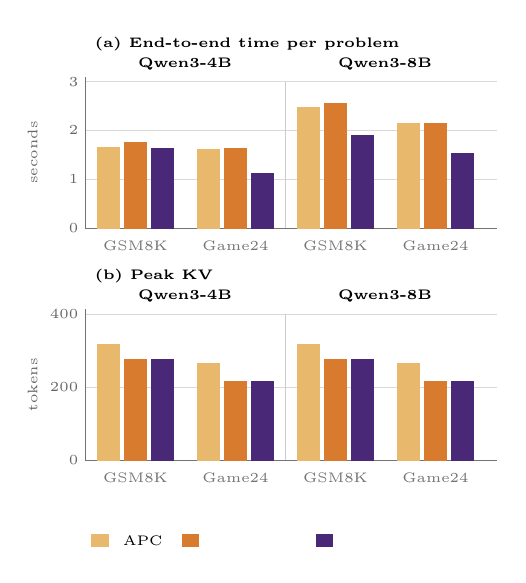
\begin{tikzpicture}[
  font=\scriptsize\sffamily,
  bar/.style={draw=black!55, line width=0.2pt},
  ax/.style={black!55, line width=0.35pt},
  grid/.style={black!15, line width=0.25pt},
  tick/.style={font=\tiny, text=black!60, inner sep=0pt},
  val/.style={font=\tiny, inner sep=0.2pt},
  wl/.style={font=\tiny, text=black!55, inner sep=0pt},
]
\definecolor{APC}{HTML}{E8B86D}
\definecolor{FS}{HTML}{D97B2F}
\definecolor{FSp}{HTML}{4A2878}

% (a) end-to-end seconds per problem. y = 0.38 + 0.62 * seconds. Axis 0--3 s.
\begin{scope}[shift={(0,2.95)}]
  \node[font=\tiny\bfseries, anchor=west] at (0.62,2.72) {(a) End-to-end time per problem};
  \draw[grid] (0.62,0.38) -- (5.85,0.38);
  \draw[grid] (0.62,1.00) -- (5.85,1.00);
  \draw[grid] (0.62,1.62) -- (5.85,1.62);
  \draw[grid] (0.62,2.24) -- (5.85,2.24);
  \draw[ax] (0.62,0.38) -- (5.85,0.38);
  \draw[ax] (0.62,0.38) -- (0.62,2.30);
  \node[tick, anchor=east] at (0.54,0.38) {0};
  \node[tick, anchor=east] at (0.54,1.00) {1};
  \node[tick, anchor=east] at (0.54,1.62) {2};
  \node[tick, anchor=east] at (0.54,2.24) {3};
  \node[tick, rotate=90, anchor=south] at (0.02,1.34) {seconds};
  \node[font=\tiny\bfseries] at (1.89,2.46) {Qwen3-4B};
  \node[font=\tiny\bfseries] at (4.43,2.46) {Qwen3-8B};
  \draw[black!20] (3.16,0.38) -- (3.16,2.24);
  % Qwen3-4B GSM8K: 1.66, 1.76, 1.63 s
  \fill[bar, APC] (0.78,0.38) rectangle (1.06,1.407);
  \fill[bar, FS]  (1.12,0.38) rectangle (1.40,1.474);
  \fill[bar, FSp] (1.46,0.38) rectangle (1.74,1.389);
  \node[wl] at (1.26,0.16) {GSM8K};
  % Qwen3-4B Game24: 1.61, 1.64, 1.13 s
  \fill[bar, APC] (2.05,0.38) rectangle (2.33,1.379);
  \fill[bar, FS]  (2.39,0.38) rectangle (2.67,1.396);
  \fill[bar, FSp] (2.73,0.38) rectangle (3.01,1.079);
  \node[wl] at (2.53,0.16) {Game24};
  % Qwen3-8B GSM8K: 2.48, 2.56, 1.91 s
  \fill[bar, APC] (3.32,0.38) rectangle (3.60,1.916);
  \fill[bar, FS]  (3.66,0.38) rectangle (3.94,1.968);
  \fill[bar, FSp] (4.00,0.38) rectangle (4.28,1.563);
  \node[wl] at (3.80,0.16) {GSM8K};
  % Qwen3-8B Game24: 2.15, 2.15, 1.52 s
  \fill[bar, APC] (4.59,0.38) rectangle (4.87,1.713);
  \fill[bar, FS]  (4.93,0.38) rectangle (5.21,1.716);
  \fill[bar, FSp] (5.27,0.38) rectangle (5.55,1.324);
  \node[wl] at (5.07,0.16) {Game24};
\end{scope}

% (b) peak KV. y = 0.38 + 0.00465 * tokens. Axis 0--400.
\begin{scope}[shift={(0,0)}]
  \node[font=\tiny\bfseries, anchor=west] at (0.62,2.72) {(b) Peak KV};
  \draw[grid] (0.62,0.38) -- (5.85,0.38);
  \draw[grid] (0.62,1.31) -- (5.85,1.31);
  \draw[grid] (0.62,2.24) -- (5.85,2.24);
  \draw[ax] (0.62,0.38) -- (5.85,0.38);
  \draw[ax] (0.62,0.38) -- (0.62,2.30);
  \node[tick, anchor=east] at (0.54,0.38) {0};
  \node[tick, anchor=east] at (0.54,1.31) {200};
  \node[tick, anchor=east] at (0.54,2.24) {400};
  \node[tick, rotate=90, anchor=south] at (0.02,1.34) {tokens};
  \node[font=\tiny\bfseries] at (1.89,2.46) {Qwen3-4B};
  \node[font=\tiny\bfseries] at (4.43,2.46) {Qwen3-8B};
  \draw[black!20] (3.16,0.38) -- (3.16,2.24);
  % GSM8K, both models: 318, 275, 275 tokens
  \fill[bar, APC] (0.78,0.38) rectangle (1.06,1.859);
  \fill[bar, FS]  (1.12,0.38) rectangle (1.40,1.659);
  \fill[bar, FSp] (1.46,0.38) rectangle (1.74,1.659);
  \node[wl] at (1.26,0.16) {GSM8K};
  % Game24, both models: 265, 216, 216 tokens
  \fill[bar, APC] (2.05,0.38) rectangle (2.33,1.612);
  \fill[bar, FS]  (2.39,0.38) rectangle (2.67,1.384);
  \fill[bar, FSp] (2.73,0.38) rectangle (3.01,1.384);
  \node[wl] at (2.53,0.16) {Game24};
  \fill[bar, APC] (3.32,0.38) rectangle (3.60,1.859);
  \fill[bar, FS]  (3.66,0.38) rectangle (3.94,1.659);
  \fill[bar, FSp] (4.00,0.38) rectangle (4.28,1.659);
  \node[wl] at (3.80,0.16) {GSM8K};
  \fill[bar, APC] (4.59,0.38) rectangle (4.87,1.612);
  \fill[bar, FS]  (4.93,0.38) rectangle (5.21,1.384);
  \fill[bar, FSp] (5.27,0.38) rectangle (5.55,1.384);
  \node[wl] at (5.07,0.16) {Game24};
\end{scope}

\fill[APC] (0.70,-0.72) rectangle (0.92,-0.56);
\node[font=\tiny, anchor=west] at (0.98,-0.64) {APC};
\fill[FS] (1.85,-0.72) rectangle (2.07,-0.56);
\node[font=\tiny, anchor=west] at (2.13,-0.64) {\sys};
\fill[FSp] (3.55,-0.72) rectangle (3.77,-0.56);
\node[font=\tiny, anchor=west] at (3.83,-0.64) {\plus};
\end{tikzpicture}
}
\caption{\textbf{Three-turn Tree-of-Thoughts} ($n{=}16$, $\mathrm{tp}{=}2$).
(a)~End-to-end seconds per problem.
(b)~Peak KV on the live spine.
\plus{} prefills one of four residuals.}
\label{fig:eval-mt}
\end{figure}
